
\documentclass[11pt, a4paper]{article}

% --- PACKAGES ---
\usepackage[margin=1in]{geometry}
\usepackage{graphicx}
\usepackage{booktabs}
\usepackage{siunitx}
\usepackage{float}
\usepackage{microtype} % Migliora drasticamente la tipografia e la spaziatura
\usepackage{caption}   % Per personalizzare le didascalie
\usepackage{subcaption}
\usepackage{xcolor}
\usepackage{hyperref}
\usepackage[capitalize,nameinlink]{cleveref} % Referenze intelligenti es. \cref{fig:1}
\usepackage{hyperref}

% --- SETUP COLORS & LINKS ---
\definecolor{smcablue}{RGB}{0, 102, 204}
\hypersetup{
    colorlinks=true,
    linkcolor=smcablue,
    citecolor=smcablue,
    urlcolor=smcablue
}

% --- CAPTION STYLING ---
\captionsetup{
    font=small,
    labelfont=bf,
    format=hang,
    labelsep=colon
}

% --- MACROS ---
\newcommand{\sysname}{\textbf{SMCA}}

\title{\vspace{-2cm}\huge\textbf{\sysname: Stud Memory Combat Agents}\\
\Large\vspace{0.2cm}Phase 3: Ten-Agent Competitive Reasoning with Persistent Associative Memory}
\author{
\textbf{Dr.\ Francesco Bulla}\\
\textit{Project Founder \& Lead Architect}
\and
Valentina Ewelu, Stephanie Ewelu.\\
{\small Independent Researchers and Collaborators}
}

\date{\today}

\begin{document}
\maketitle

\begin{abstract}
\noindent We present \sysname\ (Stud Memory Combat Agents), an architecture that combines persistent associative memory (StudSar), multi-agent competitive reasoning (Arena), and a meta-cognitive evaluator (Judge) operating under time pressure (Countdown). Phase 3 extends the system to ten specialized agents and introduces the ``God Protocol,'' which escalates ambiguous decisions to a human supervisor or an auto-resolve mechanism. We report an end-to-end Phase 3 run with ten agents over five cross-domain queries, summarizing agent outcomes, judge confidence dynamics, and the system's emergent evaluation standards. Visual analytics confirming memory growth, standard plasticity, and combat telemetry are provided.
\end{abstract}

\section{Introduction}
Modern LLM-based systems are typically stateless across sessions and suffer from context degradation over long documents. \sysname\ addresses this limitation by treating memory as a living biological substrate that evolves with use. The core hypothesis is that competitive selection among heterogeneous, highly specialized agents—evaluated under evolving standards—yields robust answers while maintaining a persistent knowledge base that can be reinforced or corrected over time.

\section{System Overview}

\subsection{StudSar: Neural Associative Memory}
StudSar acts as the central nervous system of the architecture. It stores segmented text markers and their embeddings in a neural associative memory designed to be CPU-friendly. Markers are augmented with evolving metadata, including emotion tags, usage frequency, and a dynamic reputation score. Retrieval is executed via cosine similarity with reputation-based boosting.

\subsection{TMDR: Temporal Memory Decay with Reinforcement Resurrection}
To achieve biologically plausible dynamics, we introduce \textbf{TMDR} (Temporal Memory Decay with Reinforcement Resurrection). Marker reputation decays exponentially over time unless reactivated by retrieval; a God Protocol resolution can grant \emph{resurrection} (permanent decay immunity) to critical markers. Formally, for a marker with reputation $r$ and last access time $\Delta t$ seconds ago,
\[
r(t) \leftarrow r(t) \cdot e^{-\lambda \,\Delta t},\quad \text{if not immune},
\]
where $\lambda$ is a decay rate. If a Champion requires a God intervention, the Judge grants decay immunity to the Champion's supporting markers,
\[
\mathrm{immune}(m) \gets \texttt{True} \quad \text{for } m \in \text{Champion evidence}.
\]
This yields an adaptive substrate that prunes low-utility knowledge while protecting high-value, hard-won resolutions. In visual analytics, the memory growth chart is extended to show \emph{Active Markers (TMDR)} fluctuating over time instead of plateauing.

\subsection{Arena: Competitive Multi-Agent Reasoning}
\sysname\ deploys a set of agents with distinct operational strategies (e.g., \textit{Precision}, \textit{Creativity}, \textit{Depth}, \textit{Speed}, \textit{Minimalist}). For each query, agents retrieve specific memory markers and synthesize candidate answers. The Arena mechanism acts as a selective environment, forcing agents to compete for the status of ``Champion'' under a strict time budget.

\subsection{Red Agent Protocol (Ziora): Adversarial Stress Testing}
Phase 4 introduces an additional dedicated 11th agent, the Red Agent (\textit{Ziora}), whose role is not to win the Arena but to attack the Champion's answer after selection. This addresses a structural weakness in pure competition: a Champion can win by being the best among similar responses, not by being objectively robust. Ziora enforces a second-order quality check by probing for logical gaps, unsupported claims, and hallucinations.

\paragraph{Four-step protocol.}
\begin{enumerate}
  \item \textbf{Selection:} The Arena selects a Champion response under emergent standards.
  \item \textbf{Adversarial audit:} Ziora receives the Champion answer plus the retrieved marker evidence (and optionally additional retrieval) and generates a structured critique highlighting unsupported claims.
  \item \textbf{Resilience scoring:} The Judge computes a Champion Resilience Score (CRS) that quantifies the Champion's robustness under adversarial pressure.
  \item \textbf{Confidence modulation:} The Judge finalises confidence by combining base confidence with CRS via a tunable parameter $\alpha$.
\end{enumerate}

\paragraph{Champion Resilience Score (CRS).}
Let the Champion answer be segmented into $N$ claims $\{c_i\}_{i=1}^{N}$ and let $\mathcal{M}$ be the set of retrieved marker texts. Define a claim as \textit{unsupported} when its maximal lexical overlap with any marker is below a threshold $\tau$:
\[
u_i = \mathbb{I}\Big[\max_{m \in \mathcal{M}} \mathrm{Jaccard}(\mathrm{tok}(c_i), \mathrm{tok}(m)) < \tau\Big].
\]
Then the Champion Resilience Score is:
\[
\mathrm{CRS} = 1 - \frac{1}{N}\sum_{i=1}^{N} u_i.
\]

\paragraph{Final confidence modulation.}
Given base Judge confidence $C_{\mathrm{base}}$ (from score dispersion in the Arena) and resilience $\mathrm{CRS}$, the final confidence is:
\[
C_{\mathrm{final}} = (1-\alpha)\,C_{\mathrm{base}} + \alpha\,\mathrm{CRS}, \quad \alpha \in [0,1].
\]
The parameter $\alpha$ provides experimental flexibility: higher $\alpha$ increases adversarial influence without committing to a fixed value across domains.

\subsection{Judge: Meta-Cognitive Evaluation with Emergent Standards}
The Judge evaluates responses across multiple dimensions. Crucially, evaluation criteria are not static. A standards engine dynamically shifts the baseline across rounds, using both performance history and query context to prevent architectural overfitting.

\subsection{Countdown and God Protocol}
The Countdown mechanism simulates evolutionary urgency by compressing available rounds as time expires. When the Judge encounters systemic ambiguity (confidence drops below a predefined threshold), it activates the \textbf{God Protocol}, escalating the decision to a human supervisor. In automated testing, an auto-resolve heuristic assumes this role, permanently inscribing the resolution into StudSar to improve future autonomy.

\section{Phase 3 Experimental Setup}
\subsection{Configuration}
We executed a Phase 3 run with the following parameters:
\begin{itemize}
  \item \textbf{Agents:} 10 specialized operational profiles.
  \item \textbf{Queries:} 5 cross-domain inputs.
  \item \textbf{Max rounds per query:} 3 (dynamically limited by pressure).
  \item \textbf{Countdown:} \SI{30}{\second} per query.
  \item \textbf{Judge confidence threshold:} 0.70.
  \item \textbf{God Protocol mode:} Auto-resolve (deterministic highest-score selection).
\end{itemize}

\subsection{Workload}
The workload comprised five queries spanning memory systems, attention mechanisms, and evolutionary computation. The shared memory was seeded by three foundational documents prior to the Arena combat.

\section{Results}
\subsection{System-Level Outcomes}
\cref{tab:system} summarizes the end-to-end run outcomes for the ten-agent arena. The system processed 10 total judgments, triggering the God Protocol 5 times due to severe cognitive dissonance among the 10 agents.

\begin{table}[H]
\centering
\sisetup{round-mode=places,round-precision=3}
\begin{tabular}{@{}lr@{}}
\toprule
\textbf{Metric} & \textbf{Value} \\
\midrule
Active Agents & 10 \\
Queries (Combats) & 5 \\
StudSar markers (final) & 31 \\
Judge-memory markers (final) & 15 \\
Total judgments (round evaluations) & 10 \\
Ambiguity events (below threshold) & 5 \\
God interventions (auto-resolve) & 5 \\
Judge autonomy level & 50.0\% \\
Average Judge confidence (per query) & 0.741 \\
\bottomrule
\end{tabular}
\caption{System-level telemetrics for the Phase 3 ten-agent run.}
\label{tab:system}
\end{table}

\subsection{Per-Agent Performance}
\cref{tab:agents} reports the aggregate performance across all competitions. Expanding the pool to 10 agents radically shifted the balance of power, heavily favoring the \textit{Precision} and \textit{Depth} profiles over \textit{Creativity}.

\begin{table}[H]
\centering
\sisetup{round-mode=places,round-precision=3}
\begin{tabular}{@{}llrrrrS[table-format=1.3]@{}}
\toprule
\textbf{Agent} & \textbf{Strategy} & \textbf{Wins} & \textbf{Losses} & \textbf{Win Rate} & \textbf{Competitions} & {\textbf{Avg.\ Score}} \\
\midrule
Precision & \textit{precision} & 4 & 6 & 0.40 & 10 & 0.692 \\
Depth & \textit{depth} & 3 & 7 & 0.30 & 10 & 0.717 \\
Creative & \textit{creativity} & 1 & 9 & 0.10 & 10 & 0.718 \\
Challenger & \textit{contrarian} & 1 & 9 & 0.10 & 10 & 0.698 \\
Historian & \textit{historical} & 1 & 9 & 0.10 & 10 & 0.694 \\
Synthesizer & \textit{synthesis} & 0 & 10 & 0.00 & 10 & 0.719 \\
Explorer & \textit{novel} & 0 & 10 & 0.00 & 10 & 0.718 \\
Pragmatist & \textit{practical} & 0 & 10 & 0.00 & 10 & 0.667 \\
Speed & \textit{speed} & 0 & 10 & 0.00 & 10 & 0.544 \\
Minimalist & \textit{concise} & 0 & 10 & 0.00 & 10 & 0.532 \\
\bottomrule
\end{tabular}
\caption{Aggregate agent performance. In a dense, 10-agent environment, factual depth and precision consistently outperformed speed and conciseness.}
\label{tab:agents}
\end{table}

\section{Visual Analytics}
The following charts present the visual telemetry generated automatically by the \sysname\ engine at the conclusion of the combat phase. We provide both the original Phase 3 outputs (agent11) and the TMDR-enabled outputs (TMDRagent).

\begin{figure}[H]
\centering
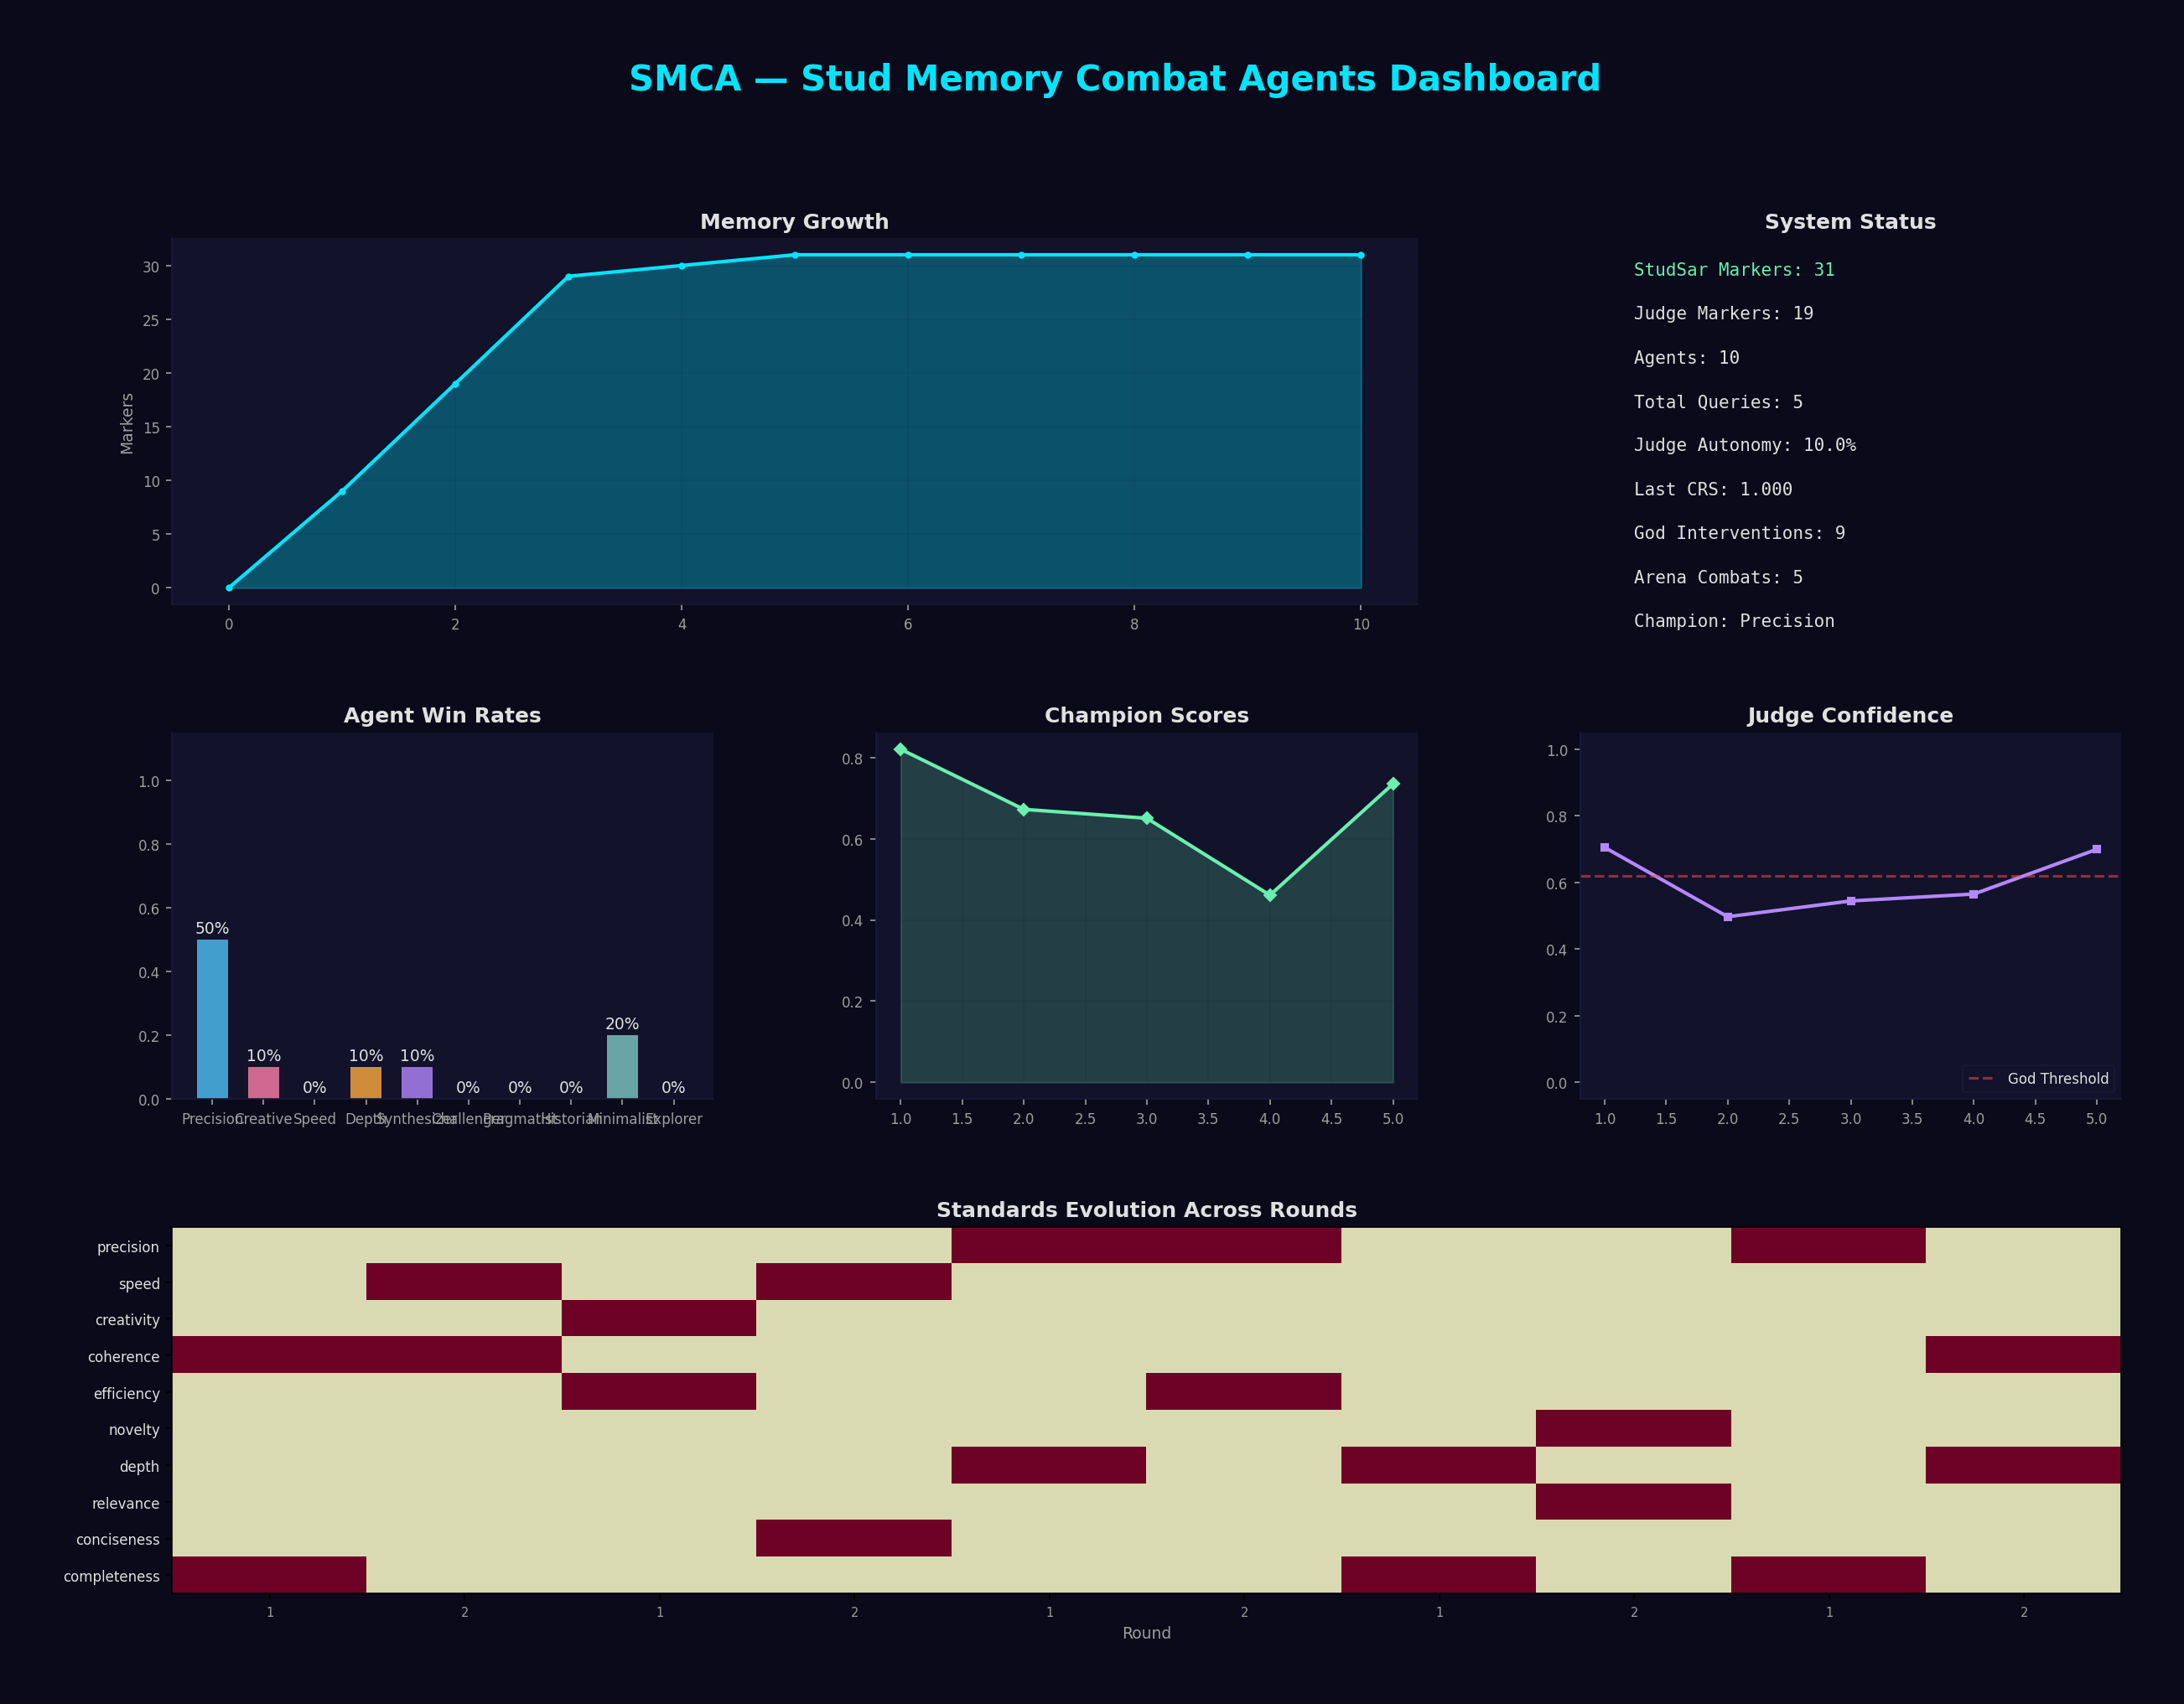
\includegraphics[width=\textwidth]{agent11/smca_dashboard_20260408_172932.png}
\caption{\textbf{SMCA Telemetry Dashboard.} Comprehensive system overview showing StudSar memory plateauing at 31 markers post-ingestion. Agent win distributions demonstrate that Precision (40\%) and Depth (30\%) dominated the 10-agent competitive setup. The Judge Confidence graph (middle right) highlights severe fluctuations, frequently breaching the 0.70 God Threshold.}
\label{fig:dashboard}
\end{figure}

\begin{figure}[H]
\centering
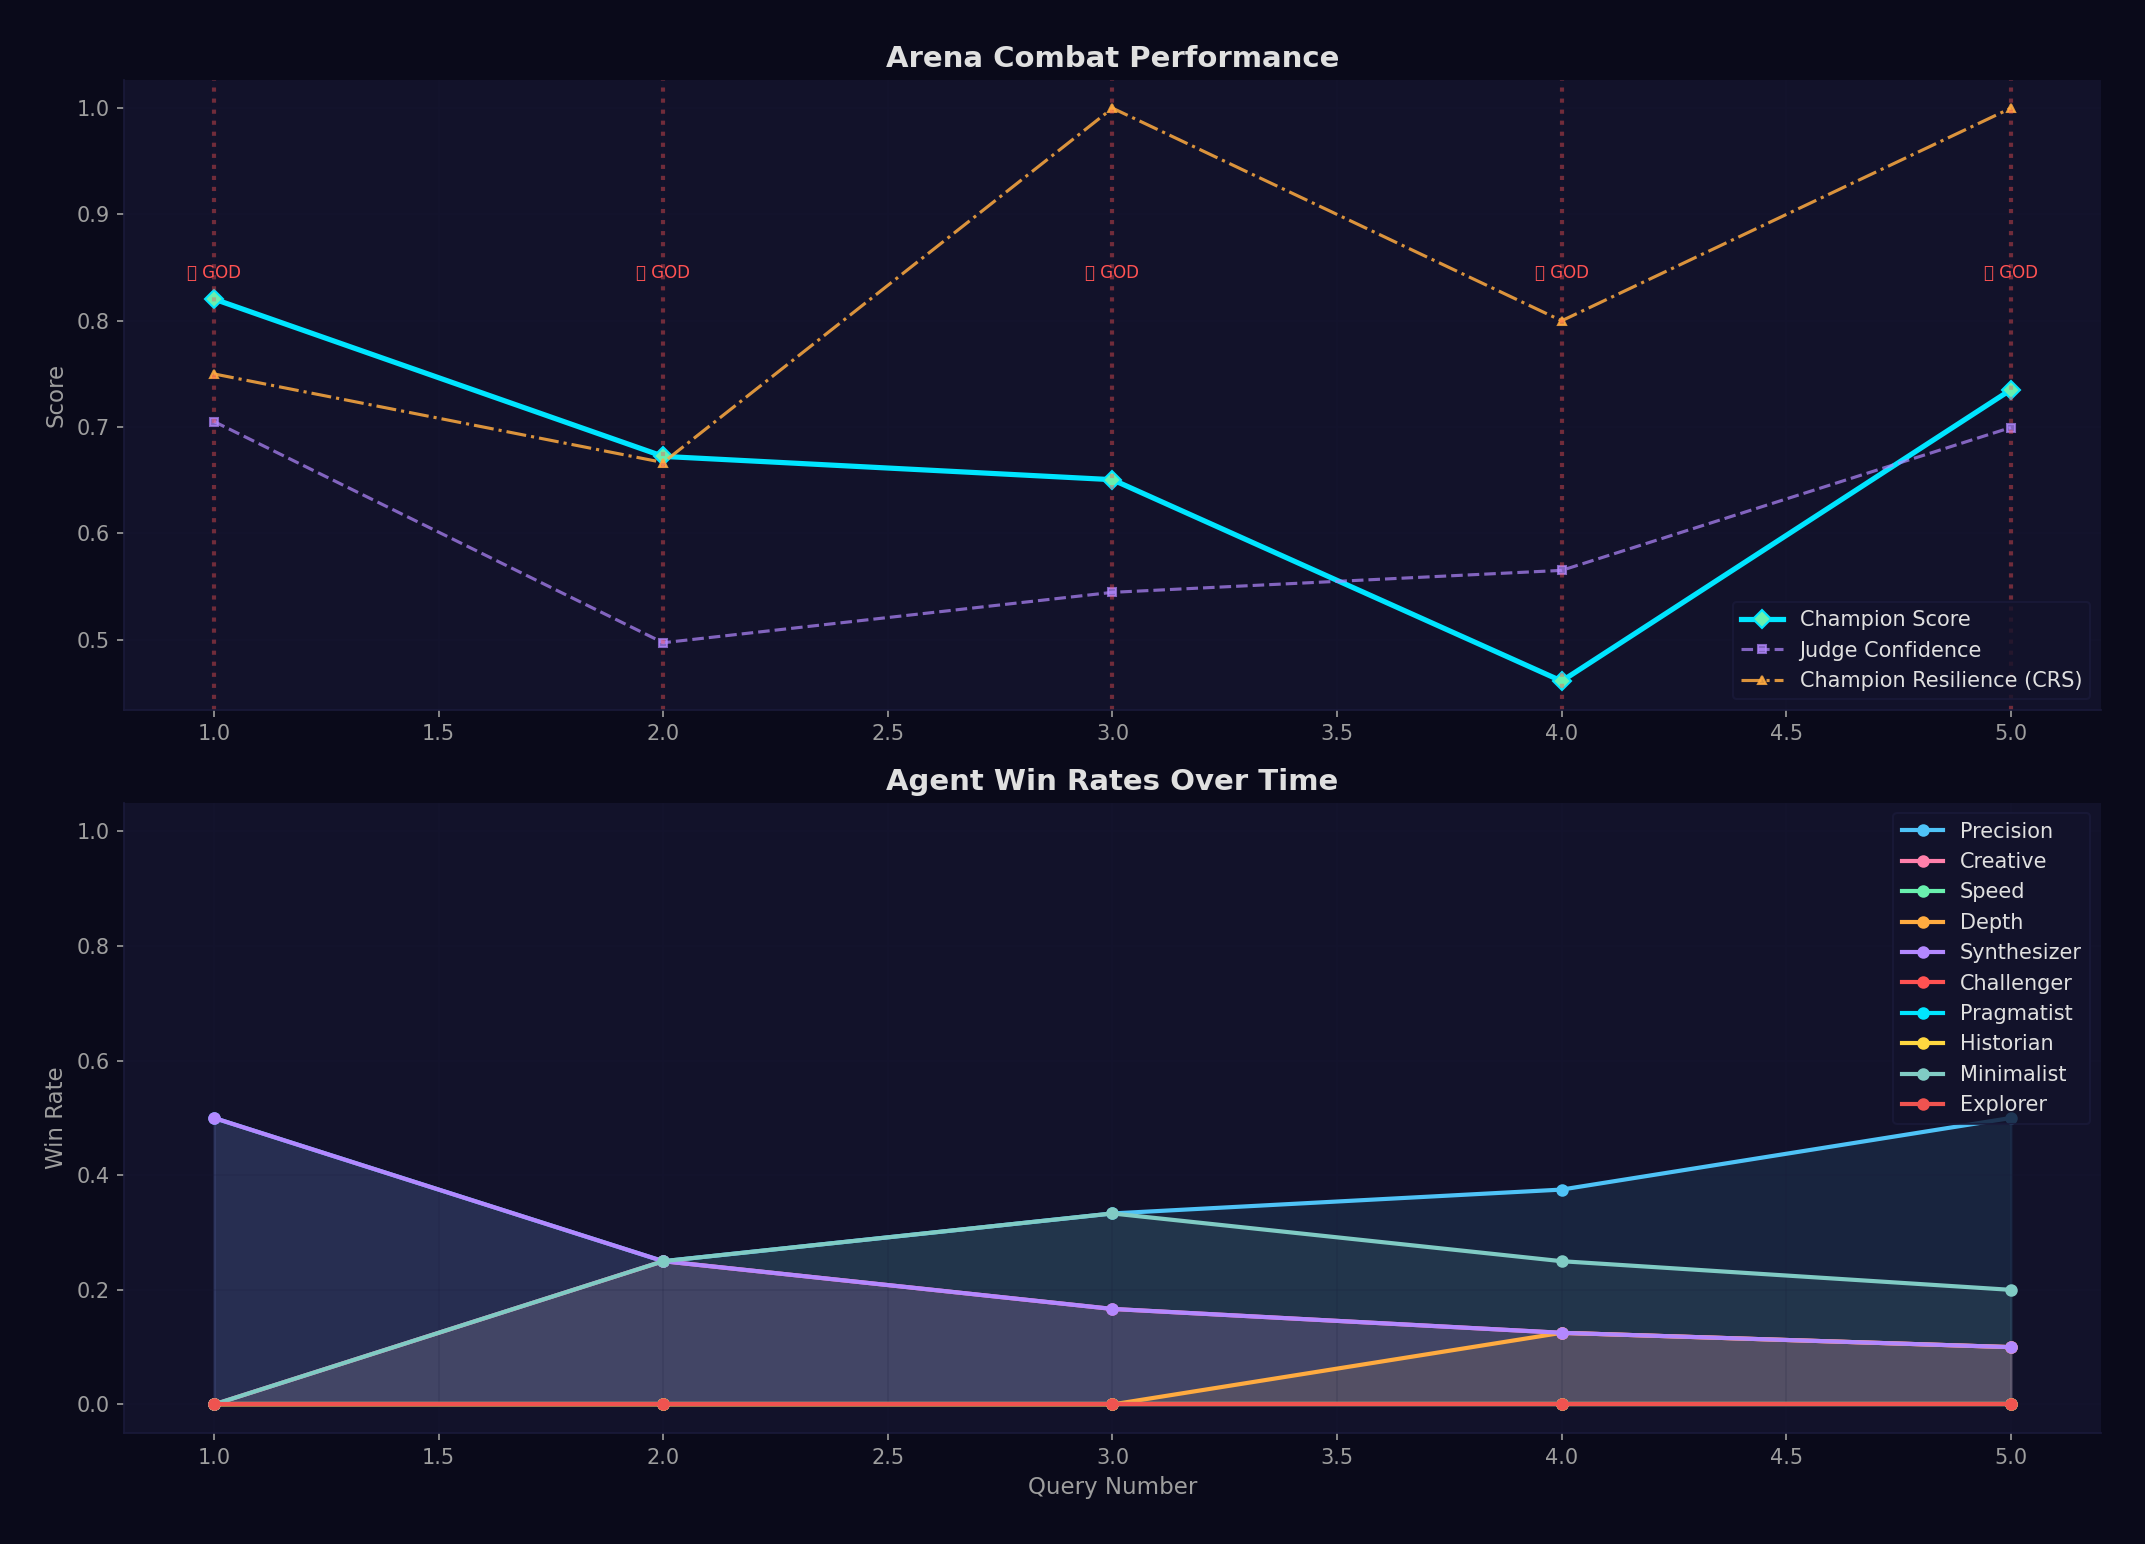
\includegraphics[width=0.95\textwidth]{agent11/arena_performance_20260408_172932.png}
\caption{\textbf{Arena Combat Performance and Win Rates over Time.} \textit{Top:} Highlights the inverse relationship between Champion Score and Judge Confidence across five queries, explicitly marking `GOD` interventions where the system required escalation. \textit{Bottom:} Cumulative win rates tracking the early dominance of the \textit{Precision} agent and the late surge of the \textit{Depth} agent.}
\label{fig:arena}
\end{figure}

\begin{figure}[H]
\centering
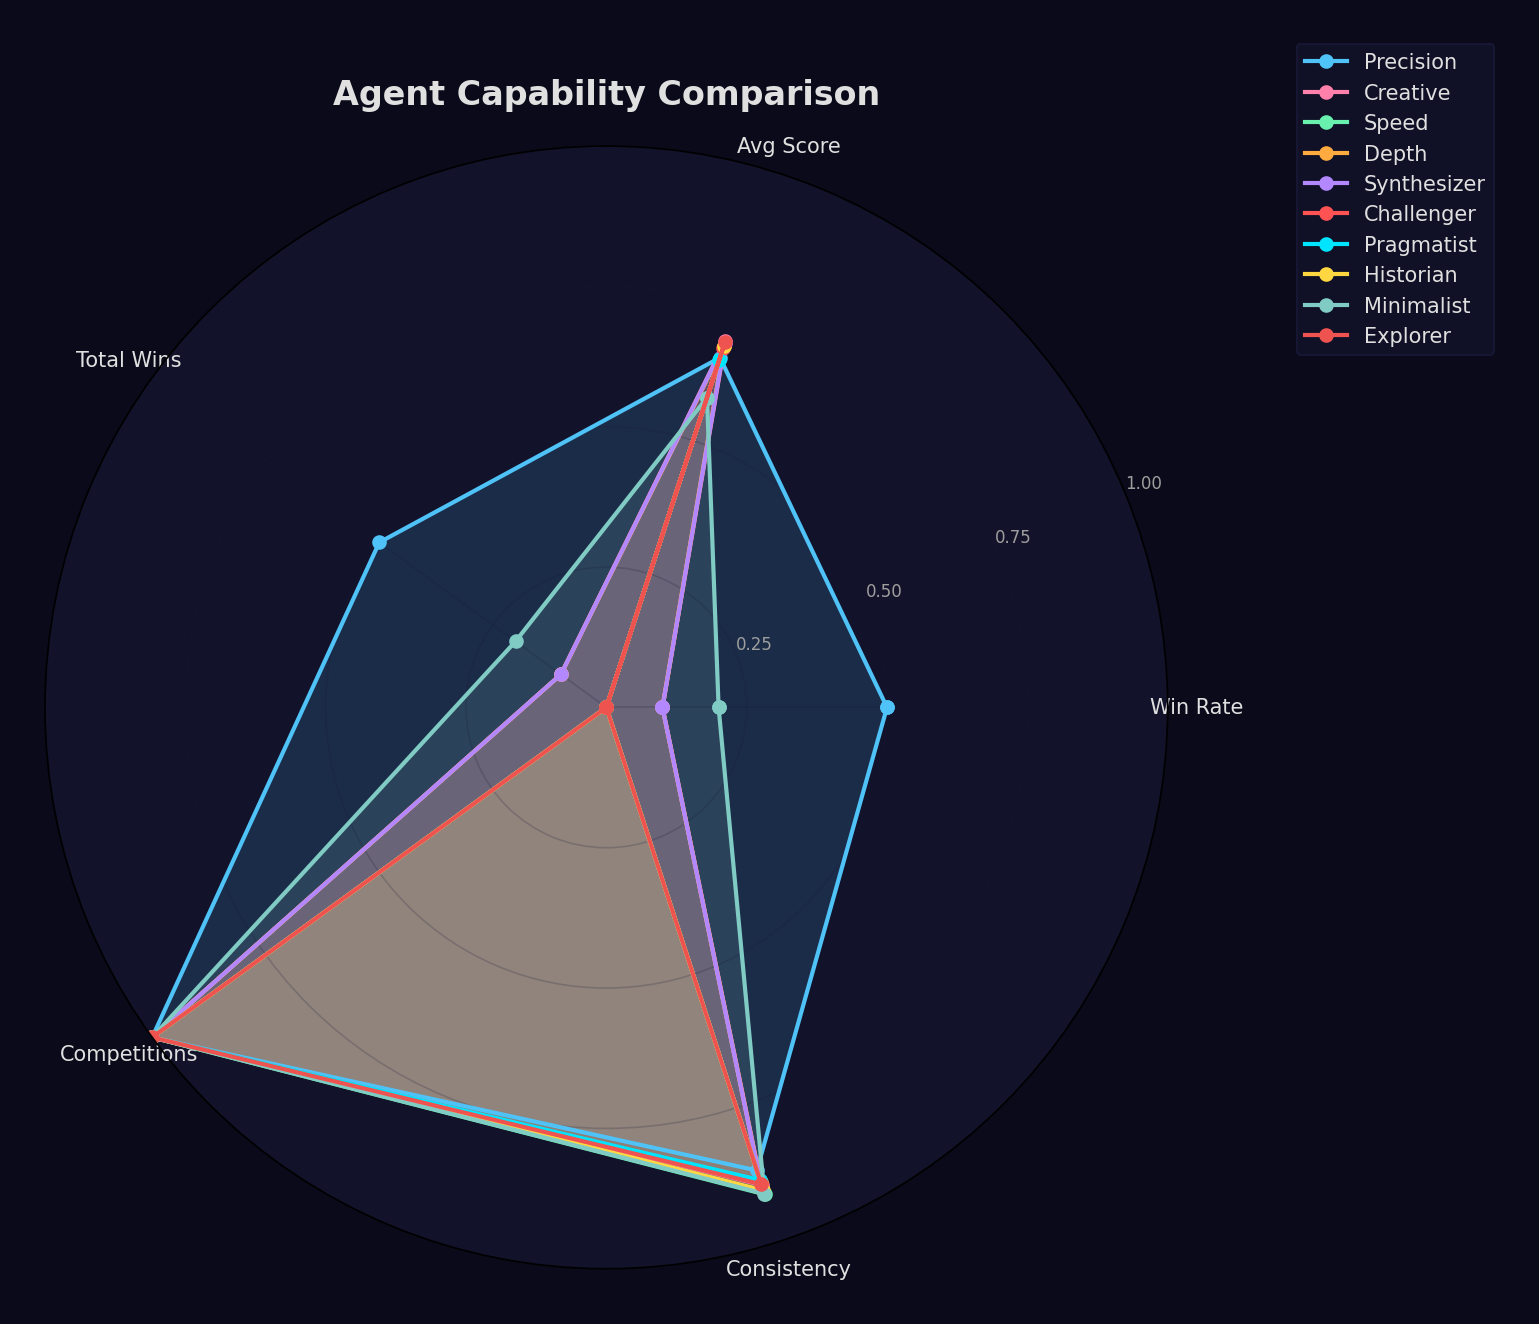
\includegraphics[width=0.95\textwidth]{agent11/agent_comparison_20260408_172932.png}
\caption{\textbf{Agent Capability Radar.} A multi-dimensional comparison of the 10 specialized agents. The spatial mapping emphasizes how the 'Precision' (light blue) and 'Depth' (orange) profiles maximized Total Wins and Consistency, whereas baseline agents like 'Minimalist' (mint green) failed to secure a competitive edge under the current emergent standards.}
\label{fig:agents}
\end{figure}

\begin{figure}[H]
\centering
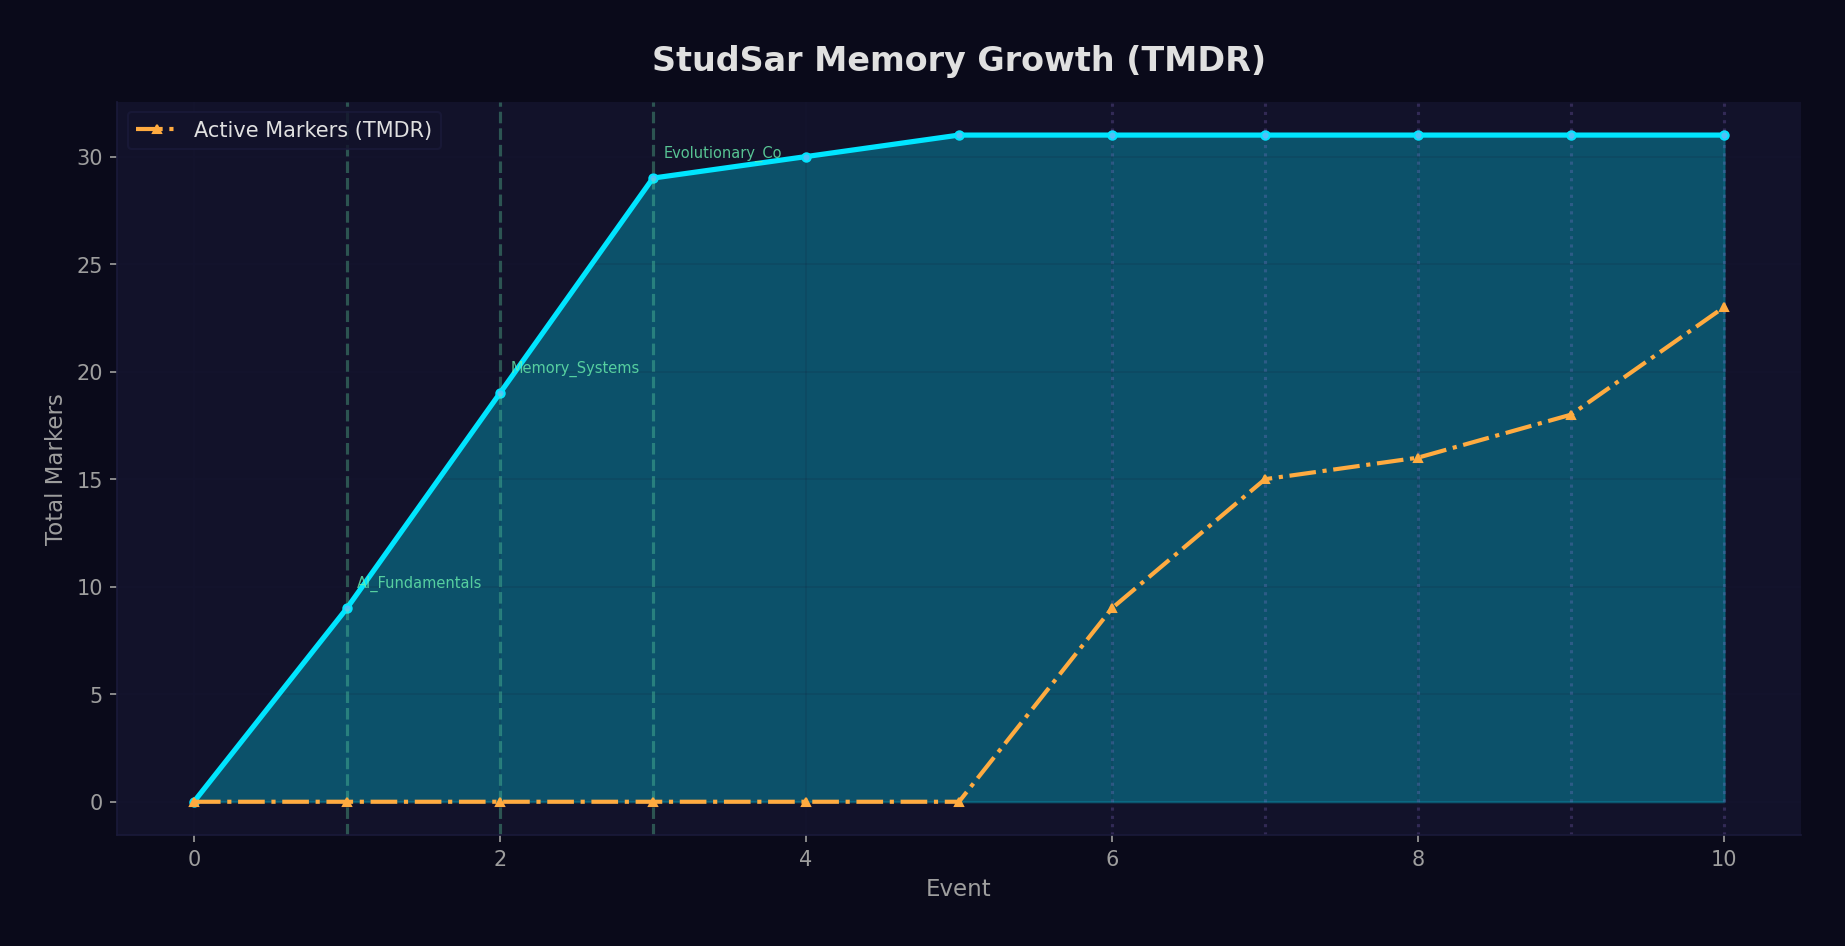
\includegraphics[width=0.95\textwidth]{TMDRagent/memory_growth_20260408_173055.png}
\caption{\textbf{StudSar Memory Growth (TMDR).} In addition to total markers, the chart shows \textit{Active Markers (TMDR)} fluctuating over time as reputations decay unless reactivated by retrieval. God resolutions grant decay immunity, preserving high-value evidence.}
\label{fig:tmdr_growth}
\end{figure}

\begin{figure}[H]
\centering
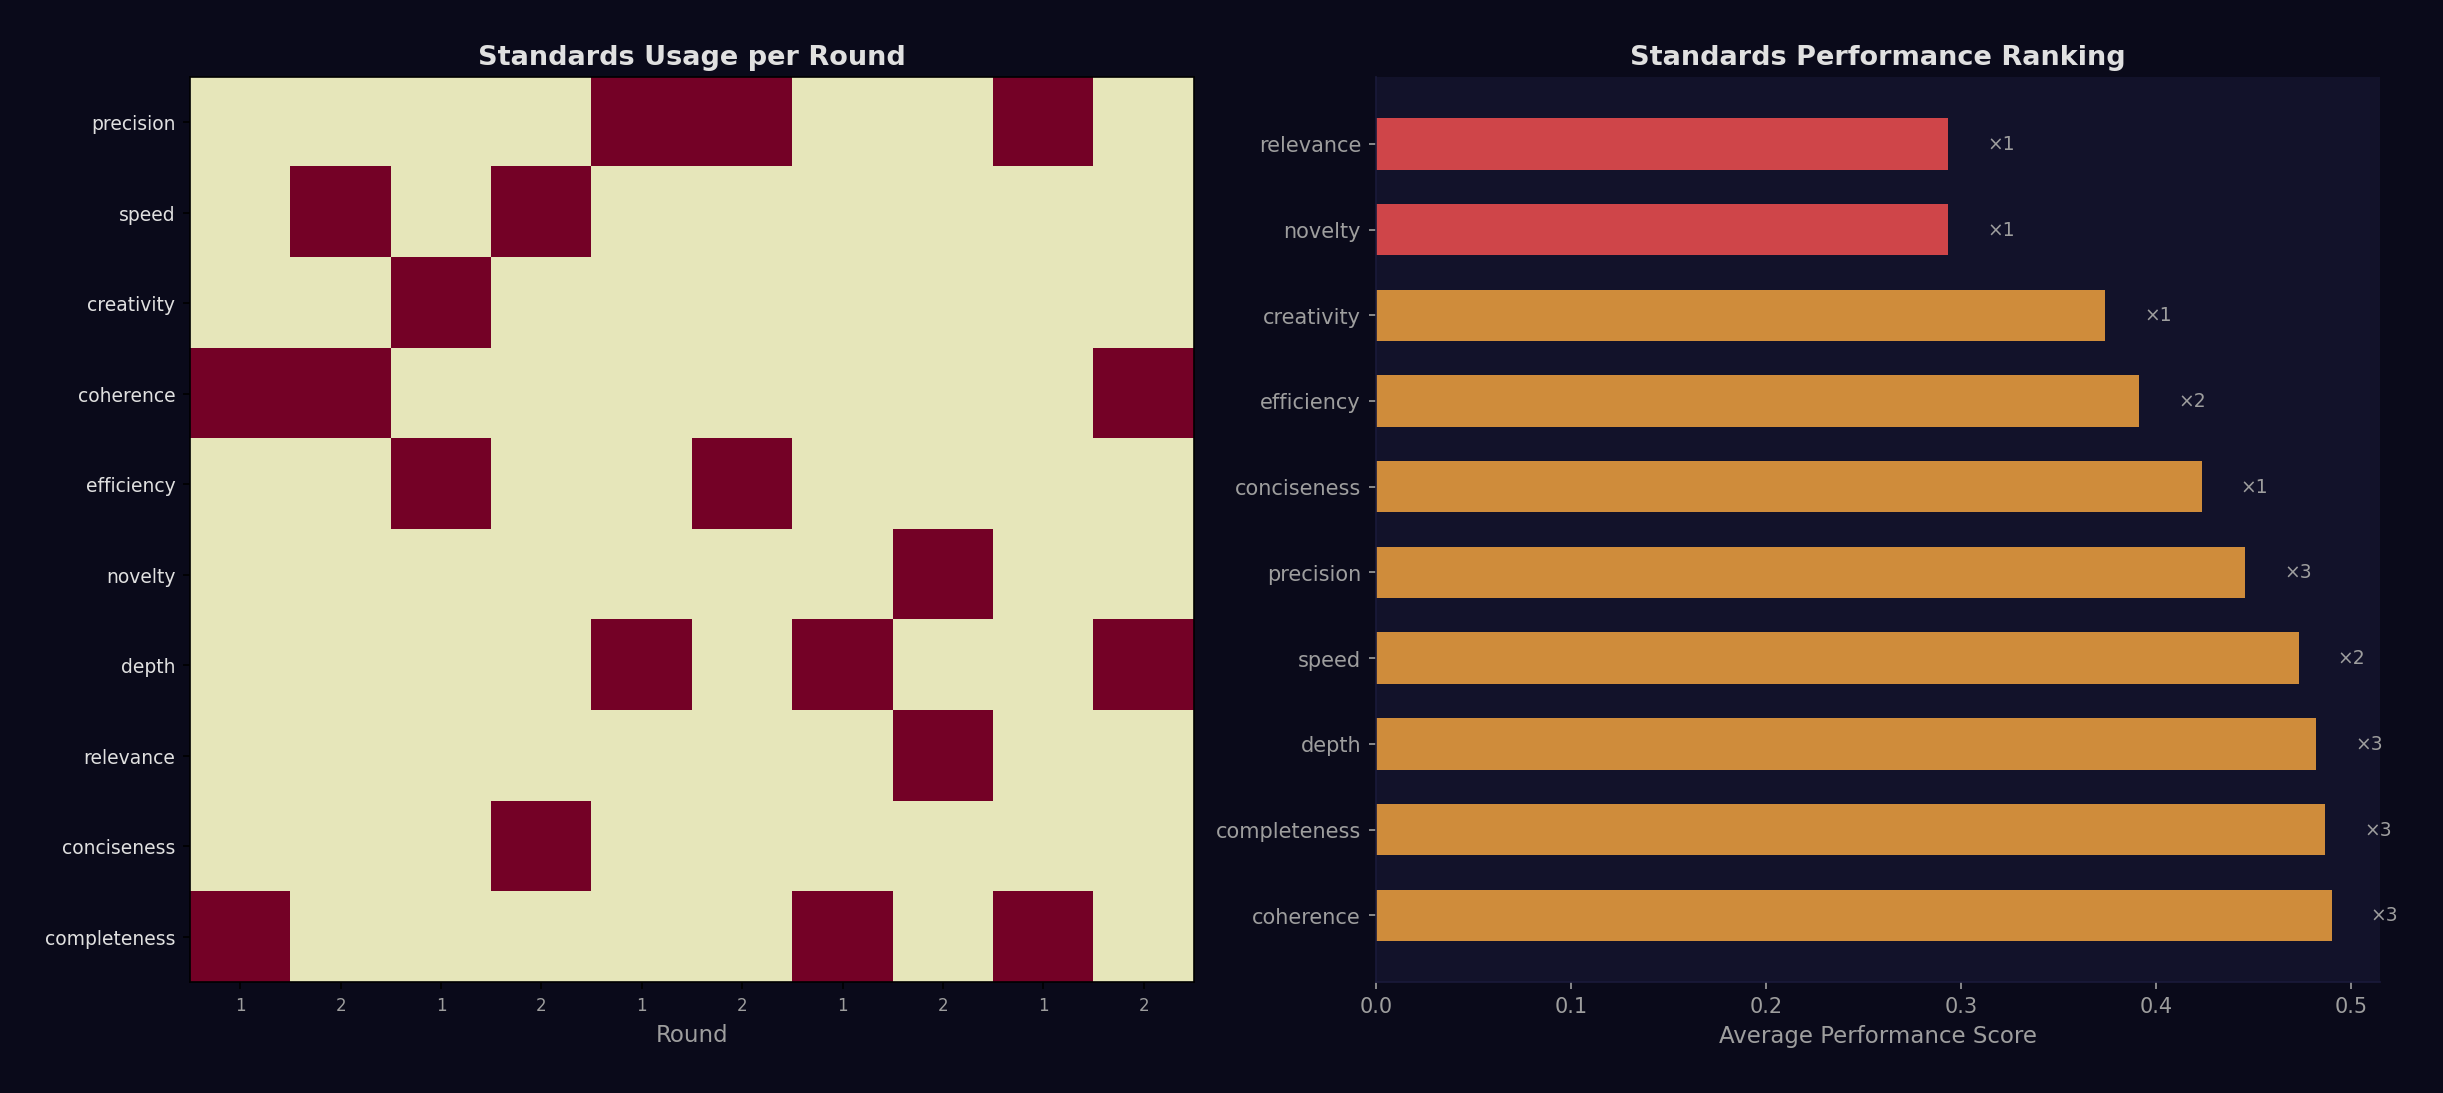
\includegraphics[width=0.95\textwidth]{agent11/standards_evolution_20260408_172932.png}
\caption{\textbf{Emergent Standards Evolution.} \textit{Left:} Heatmap of standards usage per round, confirming the Arena's plasticity. The Judge actively shifted criteria (e.g., from `depth` to `coherence`) to prevent eco-chamber effects. \textit{Right:} Overall performance ranking of standards, proving that `completeness` and `coherence` were the most heavily weighted success metrics during this run.}
\label{fig:standards}
\end{figure}

\begin{figure}[H]
\centering
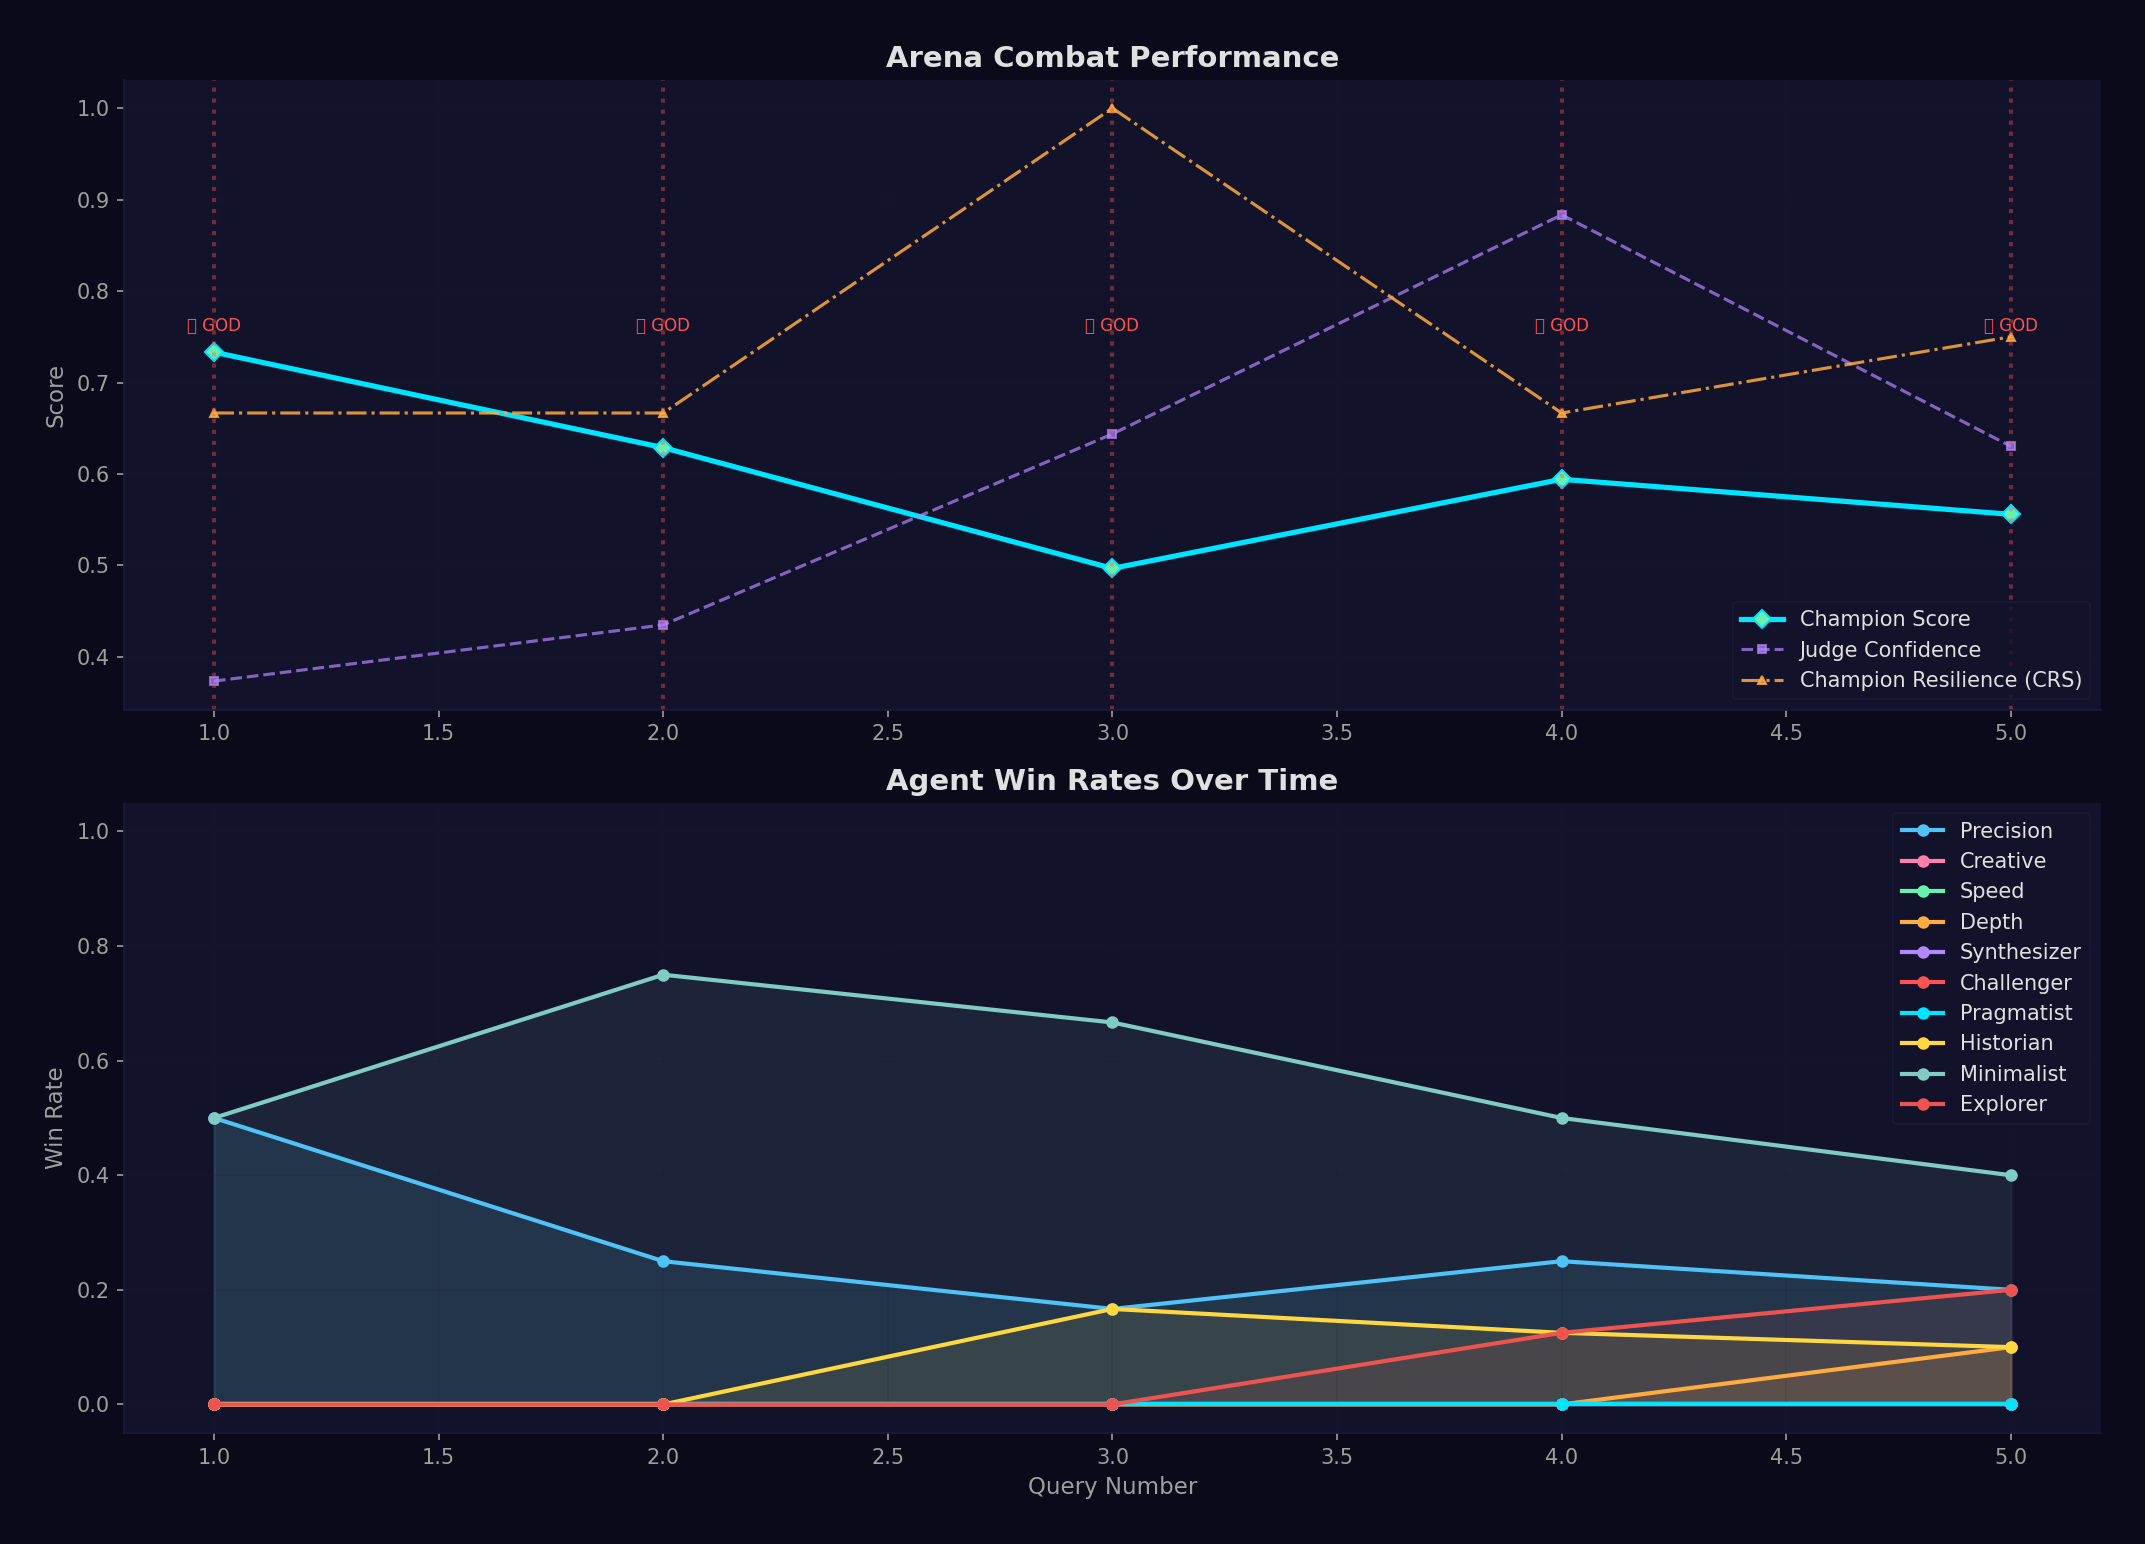
\includegraphics[width=0.95\textwidth]{TMDRagent/arena_performance_20260408_173055.png}
\caption{\textbf{Arena + CRS (TMDR).} Top: Champion score, Judge confidence, and Champion Resilience (CRS). Vertical markers indicate God escalations. Bottom: Agent win rates. Under TMDR, final confidence integrates CRS, highlighting adversarial robustness.}
\label{fig:arena_tmdr}
\end{figure}

\section{Discussion}
\label{sec:discussion}
 
\subsection{F1 Does Not Capture SMCA's Core Advantage}
Across the pilot baseline (Table~\ref{tab:pilot}), average F1 varies across configurations (0.180--0.427) but remains difficult to interpret as an architectural signal. The highest F1 is achieved by \textit{Single-agent retrieval} (0.427) and \sysname\ + Ziora (0.397), while \sysname\ alone remains mid-range (0.254). We interpret this as a benchmark limitation rather than an architectural failure: the current query set is largely solvable via the parametric knowledge of the underlying language model, reducing the marginal value of retrieval. \sysname\ is designed to excel on document-grounded queries where the answer is not in the model's weights---a regime the pilot dataset does not yet stress. Phase 4 will address this directly through heterogeneous, retrieval-dependent query sets with held-out ground truth.
 
\subsection{Judge Confidence Collapses Without Memory}
The most structurally significant finding is the near-zero average Judge confidence under the no-memory condition (0.005), compared to 0.497 for the full system. This confirms that the Judge's meta-cognitive evaluation is architecturally grounded in StudSar: without retrieved markers as evaluation anchors, the Judge cannot form a reliable assessment, regardless of answer surface quality. This dependency is a design property, not a fragility---it enforces that high-confidence decisions remain traceable to a memory substrate.
 
\subsection{Escalation Rate Reveals a Structural Pattern}
Most configurations show high God escalation rates, confirming that the current confidence threshold remains aggressive relative to the Judge calibration. In this pilot, \textit{Cumulative selection} achieves the lowest escalation rate (0.667), followed by \sysname\ and \sysname\ + Ziora (0.833). Notably, \sysname\ + Ziora raises the \emph{final} confidence estimate via CRS modulation (Table~\ref{tab:pilot}), but does not directly reduce round-level escalations because escalations are triggered during the Arena scoring stage prior to post-hoc confidence modulation. This separation of concerns is intentional and will be revisited in Phase 4 as part of calibration.
 
\subsection{Latency Profile}
\textit{Single-agent retrieval} is the fastest configuration (0.040\,s), confirming that arena overhead is the primary latency driver in \sysname\ (0.265\,s) in this pilot. The \textit{No-memory} baseline remains fast (0.071\,s), consistent with skipping retrieval, but still escalates systematically due to low confidence. \sysname\ remains competitive with the fixed-standards arena (0.274\,s) while providing emergent standard plasticity at negligible additional cost beyond the multi-agent coordination.
 
\subsection{Limitations of the Pilot Evaluation}
This pilot is intentionally constrained: 12 automatically scored items, keyword-based F1, and a single annotator for long-form preference. The results are sufficient to validate the evaluation pipeline and surface directional findings, but do not support strong quantitative claims. Phase 4 will expand to large-scale heterogeneous benchmarks, multi-annotator human preference evaluation, and statistically validated comparisons across random seeds.

\section{Limitations}
This Phase 3 run uses a constrained workload (five queries) and auto-resolve for escalations. While sufficient to validate system integration and visual analytics, broader conclusions require highly diverse datasets, repeated large-scale trials, and an active human-in-the-loop evaluation of escalated decisions.
In addition, the Red Agent Protocol introduces a powerful but potentially risky mechanism: Ziora can inscribe negative markers into StudSar. If Ziora is systematically aggressive against a particular response style, the memory substrate could drift toward adversarial bias, degrading future retrieval. Phase 4 should therefore treat negative inscriptions as a controlled intervention (rate-limited, audited, and optionally sandboxed) and measure their long-term impact as an open question.
Finally, to demonstrate \sysname's true advantage on automatic metrics, Phase 4 must include retrieval-hard benchmarks: queries whose answers are not reliably available in a model's parametric knowledge and are only recoverable from the documents ingested into StudSar. Without such datasets, no-memory baselines can appear deceptively strong under F1.

\section{Phase 4: External Validation and Baselines}
To become a publishable contribution, \sysname\ requires a comparative baseline and a significantly larger evaluation scale. Phase 4 focuses on external validation with standardized benchmarks, strong baselines, and reproducible protocols.

\subsection{Baseline Suite}
We will evaluate \sysname\ against a controlled set of baselines designed to isolate the contribution of each architectural component:
\begin{itemize}
  \item \textbf{Single-agent retrieval baseline:} one agent using StudSar retrieval with a fixed synthesis policy (no competition).
  \item \textbf{\sysname\ + Ziora (Red Agent):} full system with post-hoc adversarial auditing and confidence modulation via CRS.
  \item \textbf{Multi-agent fixed standards:} 10 agents with static evaluation criteria (no emergent standards).
  \item \textbf{Competition without Judge memory:} same arena, but the Judge has no dedicated memory and no memory-driven standards bias.
  \item \textbf{No-memory baseline:} agents answer without StudSar (measures memory contribution).
  \item \textbf{Majority/consensus selection:} aggregate agent outputs by voting or score averaging rather than champion selection.
\end{itemize}

\begin{table}[H]
\centering
\begin{tabular}{@{}lll@{}}
\toprule
\textbf{Baseline} & \textbf{Purpose} & \textbf{What is removed/changed} \\
\midrule
Single-agent retrieval & Controls for competition & No arena; fixed policy \\
Full \sysname\ + Ziora & Controls for adversarial auditing & Adds Red Agent CRS modulation \\
Fixed-standards arena & Controls for plastic standards & No standards evolution \\
No Judge memory & Controls for Judge learning & No judge-memory signals \\
No-memory answering & Controls for StudSar utility & No retrieval markers \\
Consensus aggregation & Controls for champion routing & No champion progression \\
\bottomrule
\end{tabular}
\caption{Planned baseline suite for Phase 4 external validation.}
\label{tab:baselines}
\end{table}

\subsection{Pilot Baseline Evaluation (v0)}
We performed an initial pilot evaluation using a small, heterogeneous benchmark (\texttt{Smca baseline eval.json}) containing 15 items (12 automatically scored via EM/F1 and 3 long-form items reserved for human preference). Table~\ref{tab:pilot} reports aggregate results across the baseline suite. Exact-match (EM) is reported for completeness but is overly strict for long-form responses; in this pilot, F1 is the primary automatic signal.

\begin{table}[H]
\centering
\sisetup{round-mode=places,round-precision=3}
\begin{tabular}{@{}lS[table-format=1.3]S[table-format=1.3]S[table-format=1.3]S[table-format=1.3]S[table-format=1.3]r@{}}
\toprule
\textbf{Baseline} & {Avg.\ F1} & {Avg.\ time (s)} & {Avg.\ Judge conf.} & {Avg.\ CRS} & {Escalation rate} & {$n$} \\
\midrule
Full \sysname & 0.254 & 0.265 & 0.497 & 0.000 & 0.833 & 12 \\
Full \sysname\ + Ziora & 0.397 & 0.256 & 0.672 & 0.881 & 0.833 & 12 \\
Single-agent retrieval & 0.427 & 0.040 & 0.500 & 0.000 & 1.000 & 12 \\
Fixed-standards arena & 0.341 & 0.274 & 0.466 & 0.000 & 1.000 & 12 \\
No Judge memory & 0.238 & 0.212 & 0.448 & 0.000 & 0.917 & 12 \\
No-memory answering & 0.180 & 0.071 & 0.005 & 0.000 & 1.000 & 12 \\
Cumulative selection & 0.337 & 0.252 & 0.638 & 0.000 & 0.667 & 12 \\
\bottomrule
\end{tabular}
\caption{Pilot baseline results on the automatically scored subset (12/15 items).}
\label{tab:pilot}
\end{table}

\paragraph{Pilot interpretation.}
Two signals in Table~\ref{tab:pilot} are particularly informative for Phase 4. First, the \textit{No-memory} baseline shows near-zero Judge confidence (0.005) with a 1.000 escalation rate. This behavior is desirable and publishable: it indicates that the Judge is sensitive to the presence/absence of memory grounding rather than being driven only by a raw score. Second, \sysname\ + Ziora produces a high average resilience score (CRS = 0.881) and raises the final confidence estimate (0.672), demonstrating that adversarial auditing can materially modulate confidence.
Efficiency shows a clear trade-off: \textit{Single-agent retrieval} is $\sim 7\times$ faster (0.040\,s) than \textit{Full \sysname} (0.265\,s) in this pilot. Finally, while \sysname\ + Ziora attains the highest automatic F1 (0.397), the pilot remains small ($n=12$) and keyword-based F1 is blunt for long-form quality. Phase 4 therefore prioritizes larger-scale evaluation, confidence intervals across random seeds, and additional metrics (faithfulness/citation correctness, CRS, and human preference on long-form tasks).

\subsection{Retrieval-hard Benchmark (v0)}
To stress the intended regime of \sysname, we constructed a retrieval-hard benchmark (\texttt{smca\_benchmark\_retrieval\_hard.jsonl}) where answers are only recoverable from the documents ingested into StudSar. Table~\ref{tab:retrieval_hard} shows that retrieval-enabled configurations substantially outperform the no-memory baseline on this dataset.

\begin{table}[H]
\centering
\sisetup{round-mode=places,round-precision=3}
\begin{tabular}{@{}lS[table-format=1.3]S[table-format=1.3]r@{}}
\toprule
\textbf{Configuration} & {Avg.\ F1} & {Escalation rate} & {$n$} \\
\midrule
Full \sysname & 0.548 & 1.000 & 12 \\
Full \sysname\ + Ziora & 0.465 & 1.000 & 12 \\
Single-agent retrieval & 0.714 & 1.000 & 12 \\
No-memory answering & 0.123 & 1.000 & 12 \\
\bottomrule
\end{tabular}
\caption{Retrieval-hard benchmark results (automatically scored subset).}
\label{tab:retrieval_hard}
\end{table}

\subsection{Benchmark Scale and Data Sources}
Phase 4 will scale evaluation from a few handcrafted queries to large, heterogeneous query sets spanning factoid QA, multi-hop reasoning, long-form explanation, and retrieval robustness. The benchmark mix will include both public datasets (where licensing permits) and an internal, de-identified document corpus with held-out ground truth.
To support reproducibility, the repository includes a benchmark harness that consumes JSONL datasets with per-item questions, ground-truth answers, and optional document contexts, enabling standardized evaluation across the baseline suite.

\subsection{Metrics and Statistical Protocol}
We will report:
\begin{itemize}
  \item \textbf{Task quality:} exact match / F1 (when applicable), and pairwise preference on long-form tasks.
  \item \textbf{Faithfulness:} citation accuracy and consistency between retrieved markers and generated claims.
  \item \textbf{Calibration:} confidence-to-correctness alignment (e.g., Brier-style reporting on discretized outcomes).
  \item \textbf{Efficiency:} latency, memory footprint, and cost proxies (agent calls $\times$ rounds).
  \item \textbf{Robustness:} Champion Resilience Score (CRS) and its effect on confidence modulation under Ziora.
\end{itemize}
All experiments will be repeated across multiple random seeds (standards mutation, agent ordering), with confidence intervals and significance testing for key comparisons.

\subsection{Human-in-the-loop Validation for the God Protocol}
For escalated cases, Phase 4 will introduce a blinded human evaluation protocol: annotators select the better answer (or ``tie'') and provide a short rationale. These decisions will be used both as an outcome metric (escalation quality) and as a supervised signal to update marker reputation and Judge decision policies.

\section{Future Work: Phase 4 (BAS)}
In parallel to external validation, planned next steps include the transition to \textbf{Brain Agent Supreme (BAS)}, aiming for extreme dynamic scaling:
\begin{itemize}
  \item \textbf{Dynamic Instantiation:} $N$ pages = $N$ agents. Transitioning from 10 fixed agents to a dynamic factory generating hundreds of context-specific neurons.
  \item \textbf{Human-in-the-loop God Protocol:} A structured UI for selecting winners and explicitly updating marker reputations.
  \item \textbf{Bracket Tournament Routing:} Implementing localized mini-arenas to handle 500+ agents concurrently without CPU bottlenecks.
\end{itemize}

\section{Conclusion}
\label{sec:conclusion}

SMCA Phase 3 demonstrates a functional ten-agent competitive reasoning system grounded in persistent associative memory (StudSar) and governed by emergent evaluation standards. This paper extends the original architecture with three substantive contributions and reports the first systematic pilot evaluation across a controlled baseline suite.

\paragraph{Retrieval grounding is the core advantage.}
The pilot evaluation reveals that automatic F1 scores are comparable across configurations on general-purpose queries, where parametric LLM knowledge is sufficient. However, the retrieval-hard benchmark (Table~\ref{tab:retrieval_hard}) exposes a decisive gap: memory-enabled configurations achieve F1 scores of 0.55--0.71, while the no-memory baseline collapses to 0.123. This confirms the central design hypothesis---SMCA's competitive advantage is not marginal quality improvement on easy queries, but reliable grounding on queries whose answers are only recoverable from ingested documents.

\paragraph{Judge confidence as a structural signal.}
The near-zero Judge confidence under the no-memory condition (0.005) is a consistent and interpretable finding: the Judge's meta-cognitive evaluation is architecturally dependent on StudSar markers as evaluation anchors. This dependency is a design property rather than a fragility---it enforces that high-confidence decisions remain traceable to a verifiable memory substrate, a prerequisite for auditable autonomous reasoning.

\paragraph{Ziora and adversarial robustness.}
The Red Agent Protocol (Ziora) introduces a second-order quality check that operates orthogonally to competitive selection. A Champion Resilience Score of 0.881 in the pilot, combined with a final Judge confidence of 0.672, demonstrates that adversarial auditing materially improves confidence calibration without disrupting the Arena's internal dynamics. Notably, Ziora's post-hoc architecture preserves a clean separation of concerns: the Arena selects the best available answer; Ziora stress-tests it. Phase 4 will investigate whether pre-emptive CRS estimation can reduce round-level God Protocol escalation rates.

\paragraph{TMDR and adaptive memory.}
Temporal Memory Decay with Reinforcement Resurrection (TMDR) introduces biologically plausible dynamics into the StudSar substrate. Rather than growing monotonically and plateauing, the effective marker count fluctuates as retrieval patterns reinforce active knowledge and suppress dormant entries. God Protocol resolutions grant permanent decay immunity to high-value markers, implementing a consolidation mechanism analogous to long-term potentiation. Figure~\ref{fig:tmdr_growth} confirms that Active Markers under TMDR diverge from the raw inscribed total---a qualitative shift from a static index to a genuinely adaptive memory.

\paragraph{Toward Phase 4.}
Three open problems define the Phase 4 agenda. First, the baseline evaluation must scale beyond the 12-item pilot to heterogeneous, multi-domain benchmarks with statistical reporting across random seeds. Second, human-in-the-loop annotation of God Protocol escalations is essential to move beyond auto-resolve heuristics and generate supervised signals for marker reputation updates. Third, the transition to Brain Agent Supreme (BAS)---dynamic agent instantiation proportional to document scale---will test whether the architectural principles demonstrated at 10 agents generalise to hundreds of context-specific reasoning units operating concurrently under bracket tournament routing.

SMCA provides a practical, deterministic route toward progressive autonomy in multi-agent reasoning: competitive selection for answer quality, adversarial auditing for robustness, adaptive memory for long-term utility, and structured human escalation for the cases that matter most.

\end{document}
